%% LyX 2.3.0 created this file.  For more info, see http://www.lyx.org/.
%% Do not edit unless you really know what you are doing.
\documentclass[english,12pt]{article}
\usepackage[T1]{fontenc}
\usepackage[latin9]{inputenc}
\usepackage{geometry}
\geometry{verbose,tmargin=3cm,bmargin=3cm,lmargin=2.5cm,rmargin=2.5cm}
\usepackage{verbatim}
\usepackage{float}
\usepackage{textcomp}
\usepackage{amstext}
\usepackage{amssymb}
\usepackage{graphicx}
\usepackage{esint}
\usepackage[authoryear]{natbib}
\usepackage{url}

\makeatletter
%%%%%%%%%%%%%%%%%%%%%%%%%%%%%% User specified LaTeX commands.
\usepackage{ae,aecompl}
\usepackage{lineno}

\usepackage{setspace}
\doublespacing

\makeatother

\usepackage{babel}
\begin{document}

\title{Looking for compensation at multiple scales in a wetland bird community}

\author{{\Large{}Fr�d�ric Barraquand$^{1,2,*}$, Coralie Picoche$^{1}$,
Christelle Aluome$^{1,3}$, }\\
{\Large{}Laure Carassou$^{1,4}$\& Claude Feign�$^{5}$}}

\maketitle
{\large{}\bigskip{}
}{\large\par}

{\large{}}\textsuperscript{{\large{}1}}{\large{}~University of
Bordeaux, Integrative and Theoretical Ecology, LabEx COTE B�t. B2
- All�e Geoffroy St-Hilaire, 33615 Pessac, France \bigskip{}
}{\large\par}

{\large{}}\textsuperscript{{\large{}2}}{\large{}~CNRS, Institute
of Mathematics of Bordeaux 351 Cours de la Lib�ration, 33405 Talence,
France}{\large\par}

{\large{}\bigskip{}
}{\large\par}

{\large{}}\textsuperscript{{\large{}3}}{\large{}~ISPA, Bordeaux
Sciences Agro, INRA, 33140, Villenave d\textquoteright Ornon, France}{\large\par}

{\large{}\bigskip{}
}{\large\par}

{\large{}}\textsuperscript{{\large{}4}}{\large{}~Irstea, UR EABX,
50 Avenue de Verdun, 33612 Cestas, France}{\large\par}

{\large{}\bigskip{}
}{\large\par}

{\large{}}\textsuperscript{{\large{}5}}{\large{}~PNR Landes Gascognes,
Teich Ornithological Reserve, Rue du Port BP 11 33470 Le Teich, France}{\large\par}

{\large{}\bigskip{}
}{\large\par}

{*} Corresponding author. Email: frederic.barraquand@u-bordeaux.fr

\pagebreak{}

\linenumbers
\doublespacing

\begin{abstract}
Compensatory dynamics, during which community composition shifts despite a near-constant total community size, are usually rare: synchronous
dynamics prevail in natural communities. This is a puzzle for ecologists, because of the key role of compensation to explain the relation between biodiversity and ecosystem functioning. We take advantage of a long-term wetland bird community time series of 35 years, where we suspected that compensation might occur due to changes in water levels and known trends. We find that compensatory dynamics are still rare, likely due to the synchronizing influence of climate on birds, even after considering several temporal scales of covariation (during cold or warm seasons, above or below the seasonal scale). Negative covariation in abundance at the whole community level did only appear after a management change in the reserve, and at the scale of a few months or several years. Although most research has focused on the temporal scale of compensation vs. synchrony, we found that compensation varies with taxonomic and functional scale too: compensation appeared more frequently between rather than within guilds. This suggests that compensation has more potential to emerge between broad functional groups rather between species. 

\end{abstract}
\newpage{}

\section*{Introduction}

Ecological theory suggests that within rich communities, where a number
of species can have similar functions due to their proximity in morphological
or phylogenetic space, they might exhibit compensatory dynamics \citep{gonzalez2009causes}.
Compensation occurs when individuals of some species replace individuals
of other species, either because of explicit competitive processes
or shifts in some environmental driver that change selection pressures.
This is particularly likely to occur when there is a space or resource
constraint combined with temporal environmental variability. Which
species ``win'' at any particular point in time may then depend
on the fine-grained temporal environmental variation, or just on priority
effects (i.e., who gets there first). Whatever the cause of compensatory
dynamics, its main consequences for ecosystem functioning is that
the community as a whole exhibits lower biomass variation than its
constituent species \citep{gross2013species}. Compensation is therefore
intertwined with community-level stability, at least when stability
is understood as the reciprocal of variability. By contrast, another
very frequent observed outcome on biodiversity time series is synchrony
\citep{bush_fourier_2017,usinowicz_temporal_2017}. Synchrony occurs
when all species fluctuate in phase, and therefore the biomass of
the community may not fluctuate less than its constituent parts. 

Early investigations of the frequency of synchronous vs. compensatory
dynamics focused on the variance ratio, that is, the variance of the
sum of the community biomass divided by the sum of the variance of
the component species biomasses \citep{houlahan_compensatory_2007,gonzalez2009causes}.
Unfortunately, this metric is not appropriate for communities subjected
to community-wide environmental forcing \citep{ranta_detecting_2008},
because a main environmental driver (e.g., temperature or light) may
synchronize species abundances or growth rates at some scale, creating
large variance in community-wide biomass, in spite of strongly competitive
dynamics. Further research has therefore focused on specific timeframes
where compensatory dynamics may be found (e.g., below the seasonal
scale where temperature fluctuations tend to synchronize species dynamics
\citealp{vasseur_synchronous_2014}). 

Despite this effort to look for more meaningful temporal scales in
community-level time series, temporal compensation has remained surprinsingly
elusive in the field \citep{houlahan_compensatory_2007,vasseur_synchronous_2014};
but see \citet{ernest2008zero,christensen2018long}. Most datasets
used so far to evaluate temporal compensation vs synchrony involve
planktonic organisms \citep{vasseur2007spectral,vasseur_synchronous_2014}
or terrestrial plants (\citealp{houlahan_compensatory_2007,gross2013species};
though see \citealt{bell_stability_2014}. Here, we take advantage
of a long-term bird time series record at the monthly scale (over
35 years \footnote{Considering only the years used in our analysis. Otherwise, the dataset
begins in 1973.}), in a natural reserve, that allows us to dig deeper into patterns
of synchrony, at several temporal and taxonomic or functional scales. 

Indeed, taxonomic scale should be a main modulator of synchrony/compensation,
an explanatory factor that has been somewhat neglected for now. On
the one hand, one could argue that compensation should be higher between
closely related species, because functional and phylogenetic differences
are generally correlated. For example, if species A and B are two
duck species that share almost the same food niche as well as many
traits, it makes little difference to the rest of the community whether
one species gets replaced by the other (functional compensation,\emph{
sensu} \citealt{gonzalez2009causes}), and priority effects could dominate.
On the other hand, it could be argued that these two similar duck
species will precisely respond in similar ways to environmental variables,
which tends to obfuscate compensation. Under the latter scenario,
more dissimilar species or groups of species - within the same trophic
level nonetheless - could compensate each other within the whole community,
precisely because they have different environmental preferences and
the environment varies over time (e.g., groups of species preferring
more open vs more closed habitats replacing each other as a function
of changes in vegetation height). Surprisingly, compensation between
guilds has been less well explored than within guilds, even though
there is actually some empirical evidence for compensation between
dissimilar guilds \citep{sinclair2013asynchronous}. We therefore
explore different ways to cluster the bird community, within or between
guilds, along either taxonomic or functional classifications. 

Our objective is therefore to examine how synchronous or compensatory
bird communities are at different temporal and taxonomic (or functional)
scales. Our dataset is ideally suited to the task given that (i) it
is a highly temporally resolved time series with respect to the species
typical generation times, but it also extends well beyond generation
time (35 years) and (ii) the reserve where the data has been collected
was subjected to a major management change c. 2006 (change in water
levels), favouring different types of wetland birds (so that over
long timescales, there is a real potential for changes in community
composition). 

\section*{Material and Methods}

\subsection*{Data}

The monthly time series used for the statistical analyses have been
collected at the Teich Ornithological Reserve, Arcachon Bay, France
(44.64�N / -1.02�E), by the staff of the Teich reserve. The reserve
comprises 120 ha of wetlands, and the data have been aggregated at
the reserve scale. We use for each species the maximum observed abundance
over a month, which provides a ``monthly snapshot'' of the bird
abundance. In the statistical analyses, we use both the original monthly
data and seasonal averages. We defined two seasons based on observations
of bird presence. We defined a `warm season', from May to August,
and a `cold season' as the months between November and February of
the following year. From an ecological viewpoint, this seasonal classification
separates wintering birds from summer residents (some of whom are
breeding). This makes sense biologically because the two communities
have different requirements and respond differentially to abiotic
drivers. It is also useful from a more statistical perspective, as
there is a shift in composition between the seasons, though winter
and summer communities partially overlap due to a number of shared
species. 

Fig. \ref{fig:Temporal-trends} shows the patterns in abundance for
key groups in the Teich reserve bird community, showing the marked
signature of seasonality.

\begin{figure}[H]
\begin{centering}
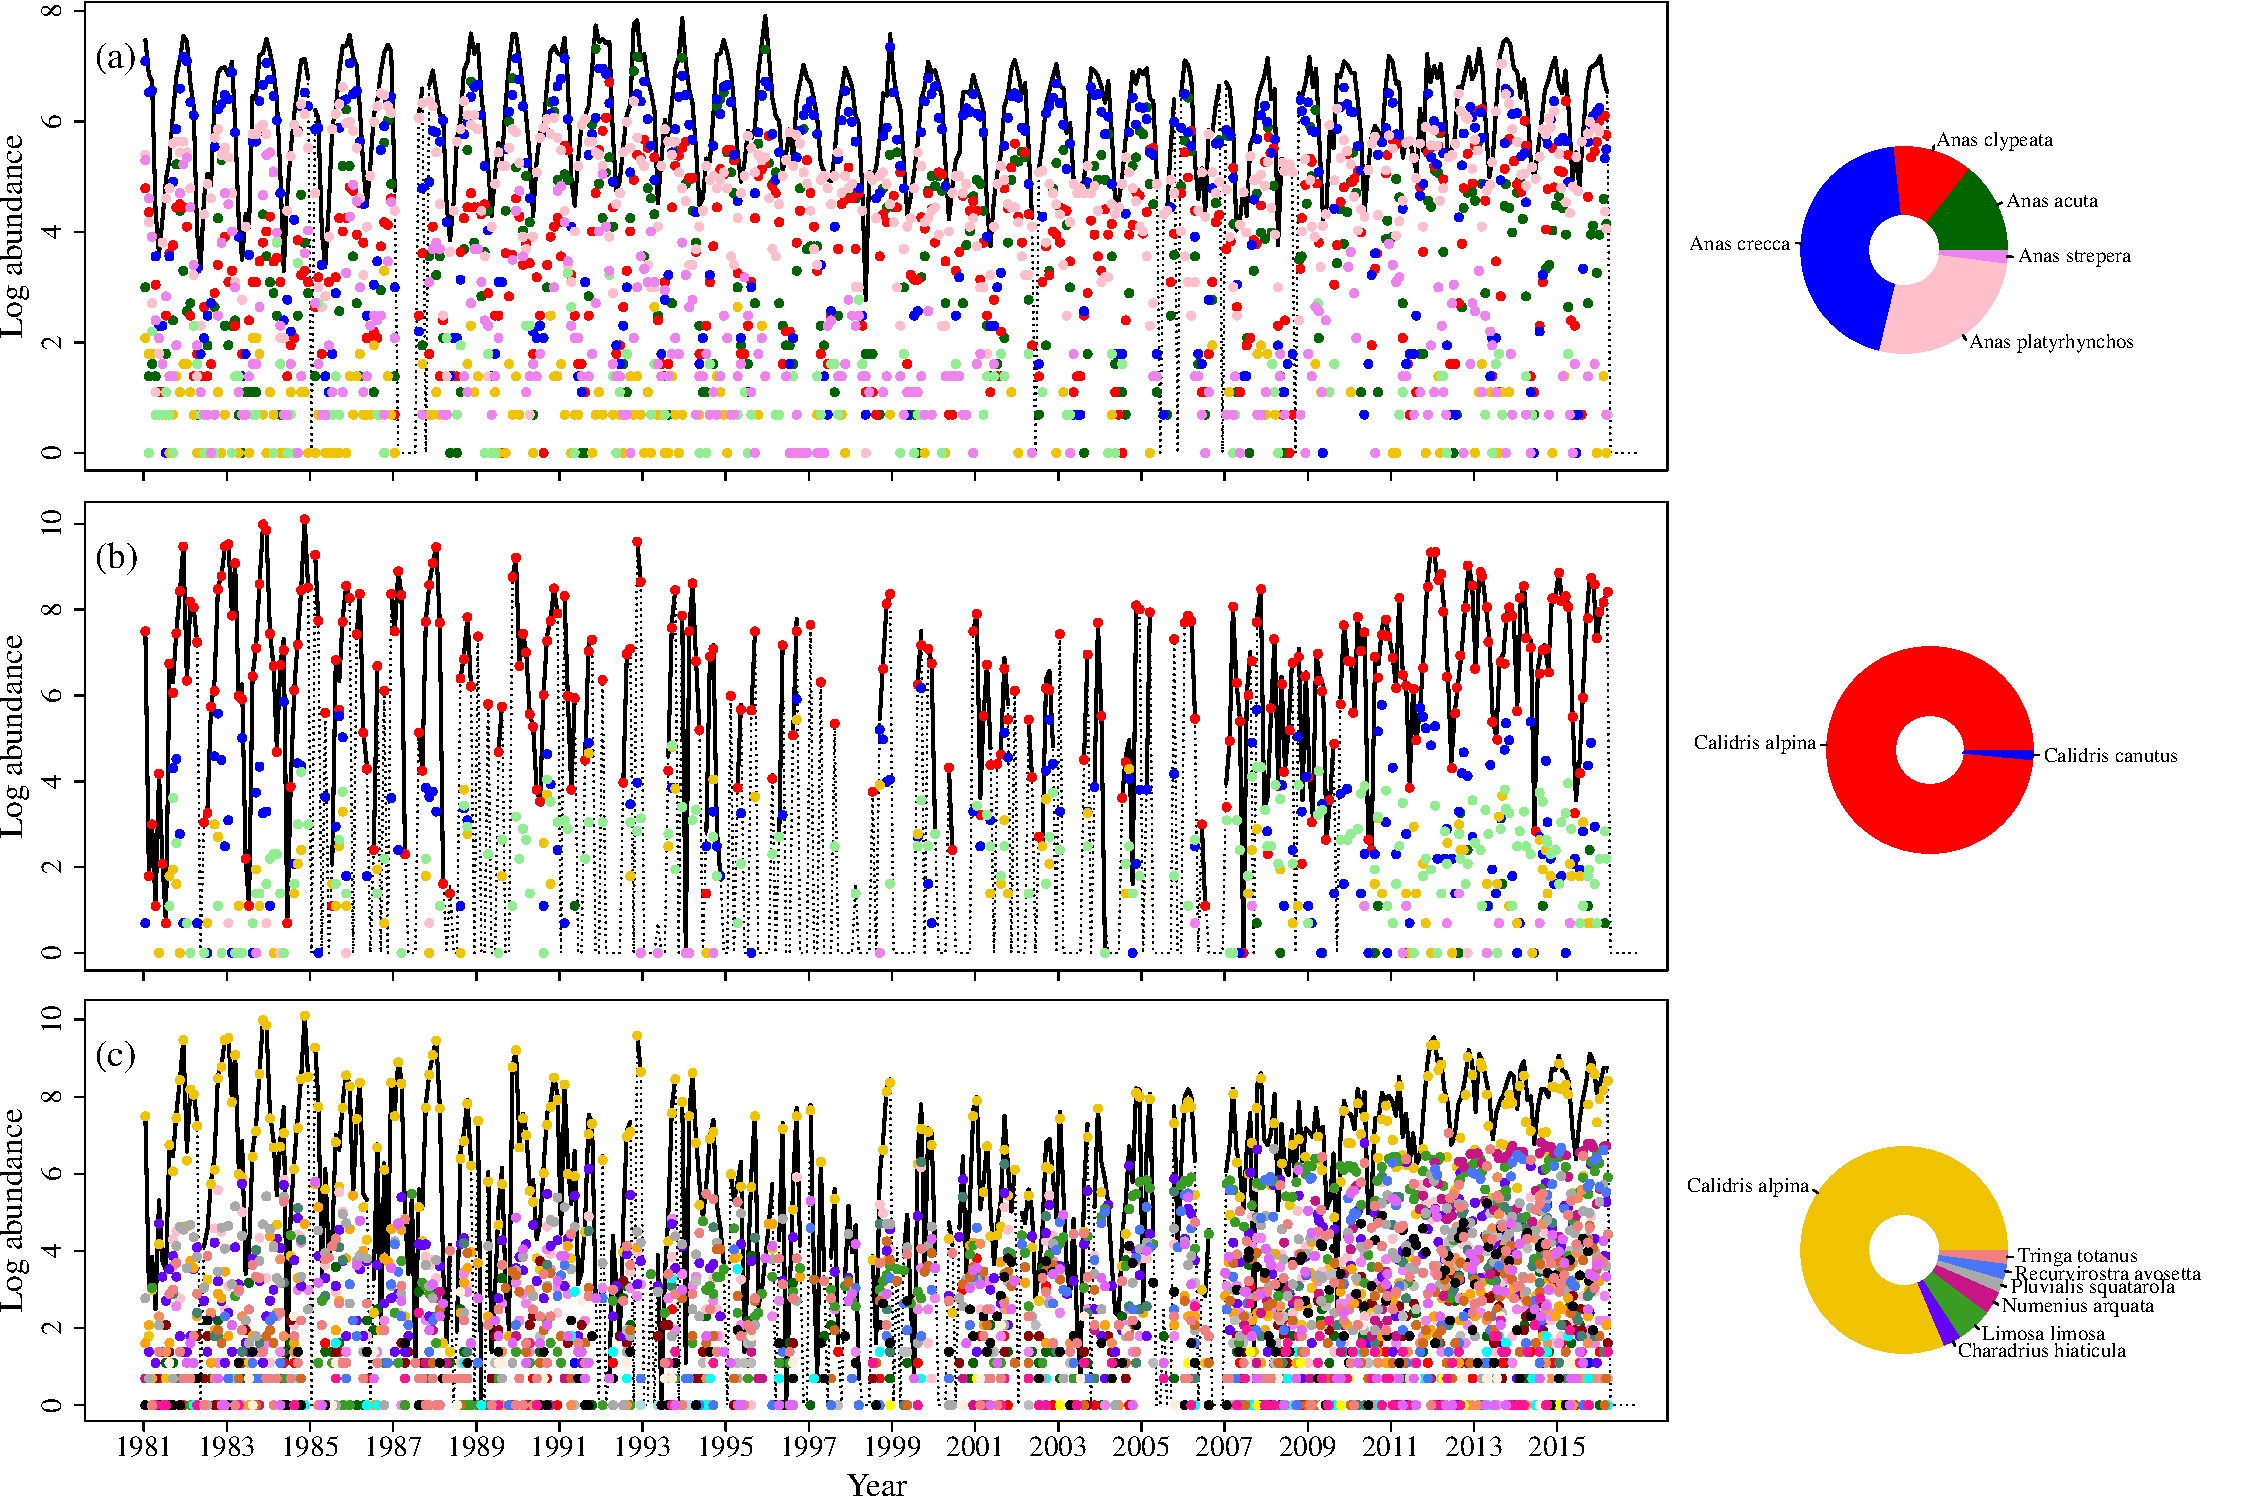
\includegraphics[width=18cm]{Fig1.pdf}
\par\end{centering}
\caption{Time series of counts for\emph{ }ducks of the genus\emph{ Anas} (a),
calidrids (b, \emph{Calidris} genus), and all waders (c, including
calidrids). The solid black lines represent trends in summed abundances
for each guild, thin dotted lines represent putative trends (when
some species are absent). The coloured symbols below the curves represent
each species abundances, with species composition on the right side
on the donut plots for the most abundant species (over 1\% of relative
abundance in the group considered). \label{fig:Temporal-trends}}
\end{figure}


\subsection*{Statistical Analyses}

We used for yearly analyses the synchrony index $\eta$ defined by
\citet{gross2013species}, which is constructed as the
mean cross-correlation between each species biomass and the summed
biomasses of the rest of the community (eq. \ref{eq:Gross}). 

\begin{equation}
\text{\ensuremath{\eta}}=\frac{1}{n}\sum_{i}\text{Corr}(P_{i},\sum_{j\neq i}P_{j})\label{eq:Gross}
\end{equation}

where $P_{i}$ is the abundance or biomass of species $i$ in a community
of $n$ species. This synchrony index described in eq. \ref{eq:Gross}
varies between -1 (perfect compensation, total biomass is constant)
and 1 (complete synchrony), while 0 represents a case where all populations
fluctuate independently. Contrary to other indices (e.g.,
\citealt{loreau_species_2008}'s $\phi$),
this index is independent from the richness $n$ of the community (or more
generally the number of system components) and its overall stability
\citep{bluthgen_land_2016,hallett_codyn_2016}. This is particularly important here
as we perform analyses at different taxonomic scales, and
therefore with a different $n$ in eq. \ref{eq:Gross}. 

We computed synchrony indices at the year $\times$ season scale (that
is, for a given cold or warm season each year) using the codyn package
in R \citep{hallett_codyn_2016}. We averaged monthly bird abundances,
for each species, over the season duration, and computed the synchrony
index using the year as our statistical unit. We also differentiated
periods before and after 2006, given that a management change occurred
within the reserve in 2006. We considered both the synchrony inside
a given group (e.g., among species of the \textit{Anas} genus) or
between groups (e.g., between the summed abundances of the 9 species
of genus \textit{Anas} and\emph{ }\textit{\emph{the sum of the 12
}}\textit{Calidris} species). In the latter case of between-groups
comparisons, we summed species together before seasonal averaging,
to consider seasonal averages of the monthly group density. 

We used both taxonomic classifications of the species (i.e., between
and within genera) and functional classifications of the species (e.g.,
30 species of waders versus 34 species of ducks) as we suspected that
a functional classification may allow to partition better the abiotic
requirements of the species. We use ``duck'' as a shorthand for
the larger functional group of herbivorous divers, because the birds
in that category are mostly ducks: this group includes nonetheless
all anatids (geese and swans in particular) as well as the common
coot \emph{(Fulica atra}, an abundant species here). 

We also ``zoomed in'' on a group of species that were known to exhibit
potentially compensatory dynamics (through competition for roosting
sites): the great cormorant \textit{(Phalacrocorax carbo)}, the little
egret (\textit{Egretta garzetta}) and the grey heron (\textit{Ardea
cinerea}). The little egret and the grey heron abundances were summed
because of their similar requirements (i.e., they form a small functional
group). 

We computed statistical significance of synchrony index values using
Monte Carlo randomizations \citep{gouhier_synchrony_2014}. For each
set of time series (each combination year $\times$ season), we kept
the auto-correlation of the species time-series, but removed the cross-correlation
between species by shifting each time series by a random lag \citep{purves_fine-scale_2002}.
We obtained 100 sets of randomized time series for each season and
period of time considered and computed the corresponding synchrony
index. We then compared the observed values of $\eta$ to the values
obtained with the randomized time-series. Independence of species
was rejected at the Bonferroni-corrected 10\% threshold.%
\begin{comment}
Do we Bonferronni-correct? In this case, 5/16 for the 4 seasons? (4
groups/4 season?)Do we add the equation for the p-value? Doesn't feel
necessary to me but what do you think? We'll discuss for the Bonferroni,
but that makes sense if we do it below? In any case we don't need
to mention more here if we add the codes to the GitHub repo. I don't
Bonferroni-correct for now. Thinking about it, wouldn't it be 5/(3{*}6{*}2)
(3 periods of time, 6 groups, 2 seasons) ? Bonferroni corrections
might be too strong in this context, let's discuss that together.
F: Perhaps we should Bonferroni correct after all, see my comments
on the Appendix.
\end{comment}

In addition to the time-domain analyses above, we performed frequency-domain
analyses, in particular for analyzing synchrony within the rich wader
community, as well as the group formed by the great cormorant, grey
heron and little egret. Based on the work by \citet{keitt_coherent_2008}
and follow-up by \citet{vasseur_synchronous_2014},
we used the wavelet transform of the time series to measure the coherency
between time series

\begin{equation}
\rho(t,s)=\frac{\Lambda_{t,s}(|\sum_{k}w_{k}(\tau,s)|)}{\Lambda_{t,s}(\sum_{k}|w_{k}(\tau,s)|)}\label{eq:Keitt}
\end{equation}

where $w_{k}(\tau,s)$ is the continuous Morlet wavelet transform
of species $k$ at time $\tau$ for scale $s$, $\Lambda_{t,s}(\centerdot)=\int_{-\infty}^{+\infty}e^{-\frac{1}{2}(\frac{t-\tau}{s})^{2}}(\centerdot)d\tau$
and $|\centerdot|$ is the modulus of the complex number. The numerator
corresponds to the total biomass variation while the denominator corresponds
to the variations of each species. This index is close to 0 when species
compensate and reaches 1 when they are synchronous. As before, the
significance of each value was tested at the 10\%, Bonferroni-corrected,
threshold by 100 phase-randomizations of each species time series,
and computation of the corresponding $\rho$ values.

All datasets and statistical analyses are available in a GitHub repository \url{https://github.com/fbarraquand/BirdTimeSeries_Teich} \footnote{Made public upon acceptance and archived in Zenodo}.

\section*{Results}

Using a taxonomic classification of the community (\textit{\emph{focusing
on the genera}} \textit{Calidris} and \textit{Anas} as two key examples
of contrasted birds), we can see that within-genus synchrony indices
at the seasonal scale are always positive whenever significantly different
from the null (no temporal correlation between species), i.e. there
is no compensation within a genus (Fig. \ref{fig:Gross-synchrony-index}).
This matches the patterns obtained within the entire wetland bird
community (Fig A1 in Appendix 1). 

For the cold season, \textit{Calidris} and \textit{Anas} exhibit opposite
trends in synchrony in response to the management change in 2006.
However, for the warm season, the management change, which consisted
in lowering the water levels, created more synchronous communities
of species within the \emph{Anas} and \emph{Calidris} genera. This
increase in synchrony after 2006 is matched by the functional group
classification. 

Even though there is no widespread community-wide or genus-wide compensation
at the yearly timescale (differentiating the seasons), there could
be compensation at finer temporal scales, e.g. a month or two, or
coarser scales, over several years. The wavelet plot (Fig. \ref{fig:Wavelet-modulus-ratio}),
that allows to consider a time-varying and scale-dependent strength
of synchrony, suggests that there is synchrony even at a fine temporal
scale throughout most of the time series. However, post-2006, there
seems to be a possibility for overcompensation on a scale around 5
years or around 3-4 months. 

\begin{figure}[H]
\begin{centering}
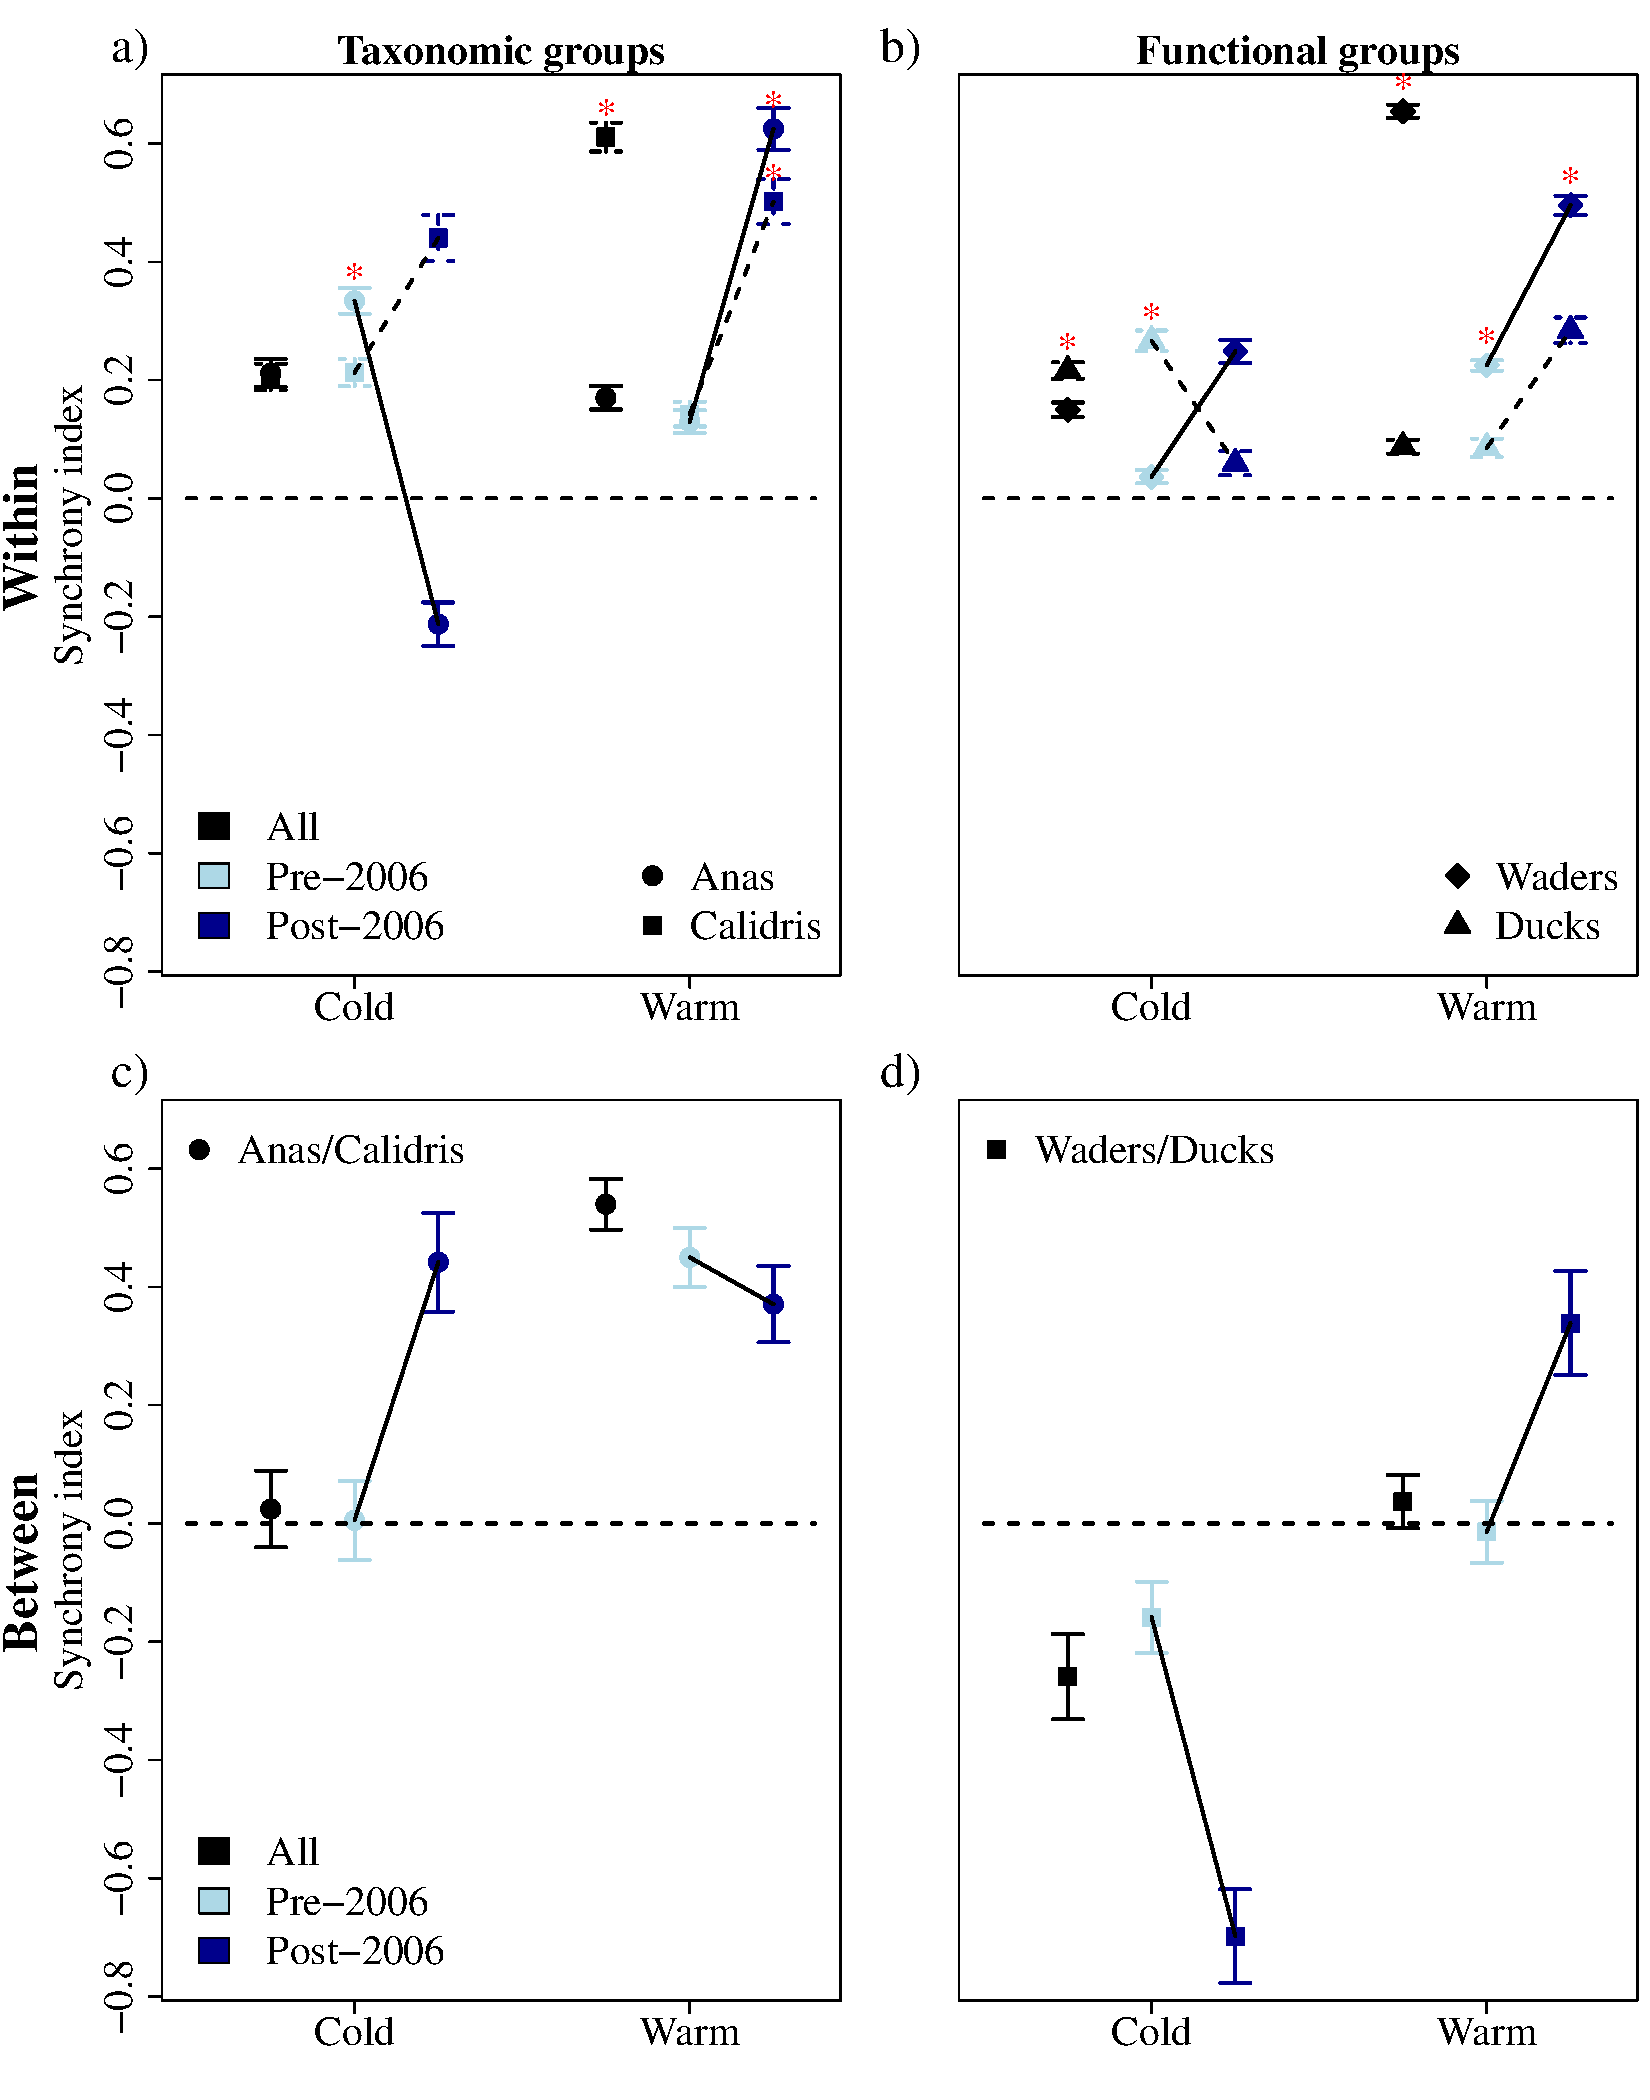
\includegraphics[width=0.85\textwidth]{Fig2_new2}
\par\end{centering}

\caption{Gross' synchrony index ($\eta$) as a function of the season (cold
and warm seasons), calculated within (top, a-b) and between (bottom,
c-d) groups. The groups considered were different functional groups
(ducks vs. waders, right b-d) or taxonomic groups (\emph{Anas} genus,
\emph{Calidris} genus, left a-b) groups. The index was computed in
each panel on the whole dataset (black) or using two periods: before
and after 2006 (light and dark blue), the year of the change in water
level management. Red stars correspond to synchrony values significantly
different from the null model (independent species), at the 10\% threshold.
\label{fig:Gross-synchrony-index}}
\end{figure}

There are therefore relatively contrasted results regarding the effect
of the management change on short-term synchrony within the wader
community. At the yearly (season) timescale, it seems to increase
the synchrony (though the Gross index and wavelets provide slightly
different answers). At even shorter timescales though, it seems to
decrease it. 

More clear-cut results can be found when we examine the synchrony
vs. compensation between functional groups (Fig. 2d). Since we consider
only two functional groups, the Gross index reduces to a simple correlation\footnote{It should be noted that with more species, the \citet{gross2013species}
index has been specifically designed so as to be able to take the
value -1 when there is a zero-sum dynamics, i.e., perfect compensation,
unlike the classical correlation coefficient. }. Waders and ducks are negatively correlated during the cold season
and positively correlated during the warm season. These patterns are
in contrast unclear when using a taxonomic classification (no compensation,
Fig. 2c).
\begin{figure}[H]
\begin{centering}
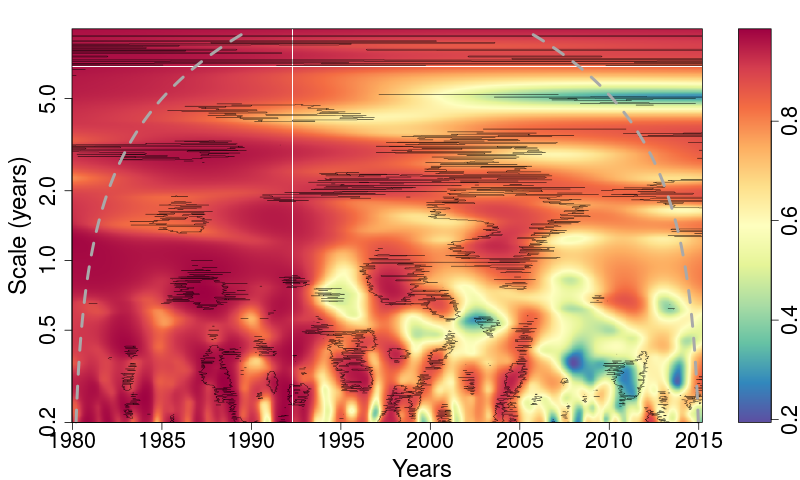
\includegraphics[width=0.95\textwidth]{Figure3}
\par\end{centering}
\caption{Wavelet modulus ratio for the wader community, scaling from 0 (compensation,
blue color) to 1 (synchrony, red color). Dashed black lines delineate
regions significantly different from the null model with a false discovery
rate controlled at the 10\% threshold. \label{fig:Wavelet-modulus-ratio}}
\end{figure}

\begin{figure}[H]
\begin{centering}
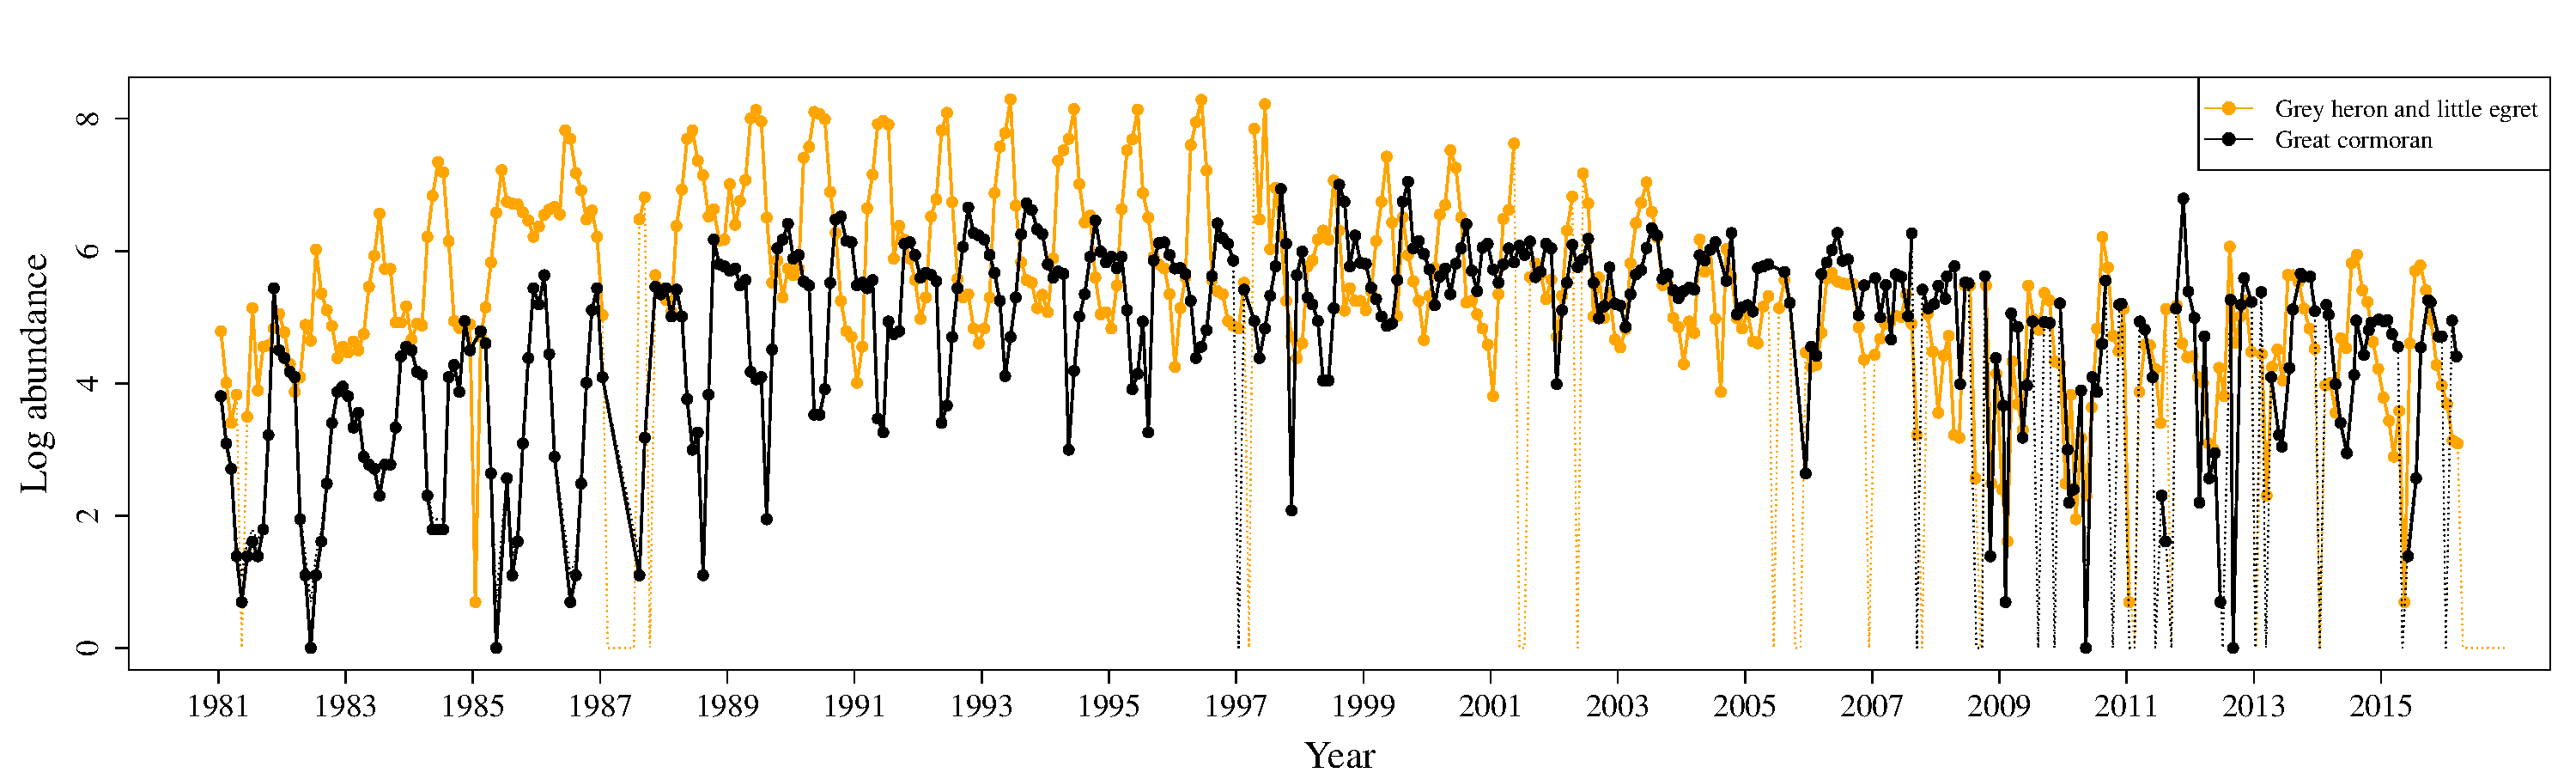
\includegraphics[width=1.1\textwidth]{Fig4}
\par\end{centering}
\caption{Time series of great cormoran abundance, as well as summed abundances
of grey heron and little egret (logarithmic scale). \label{fig:Time-series-of}}
\end{figure}

\begin{figure}[H]
\begin{centering}
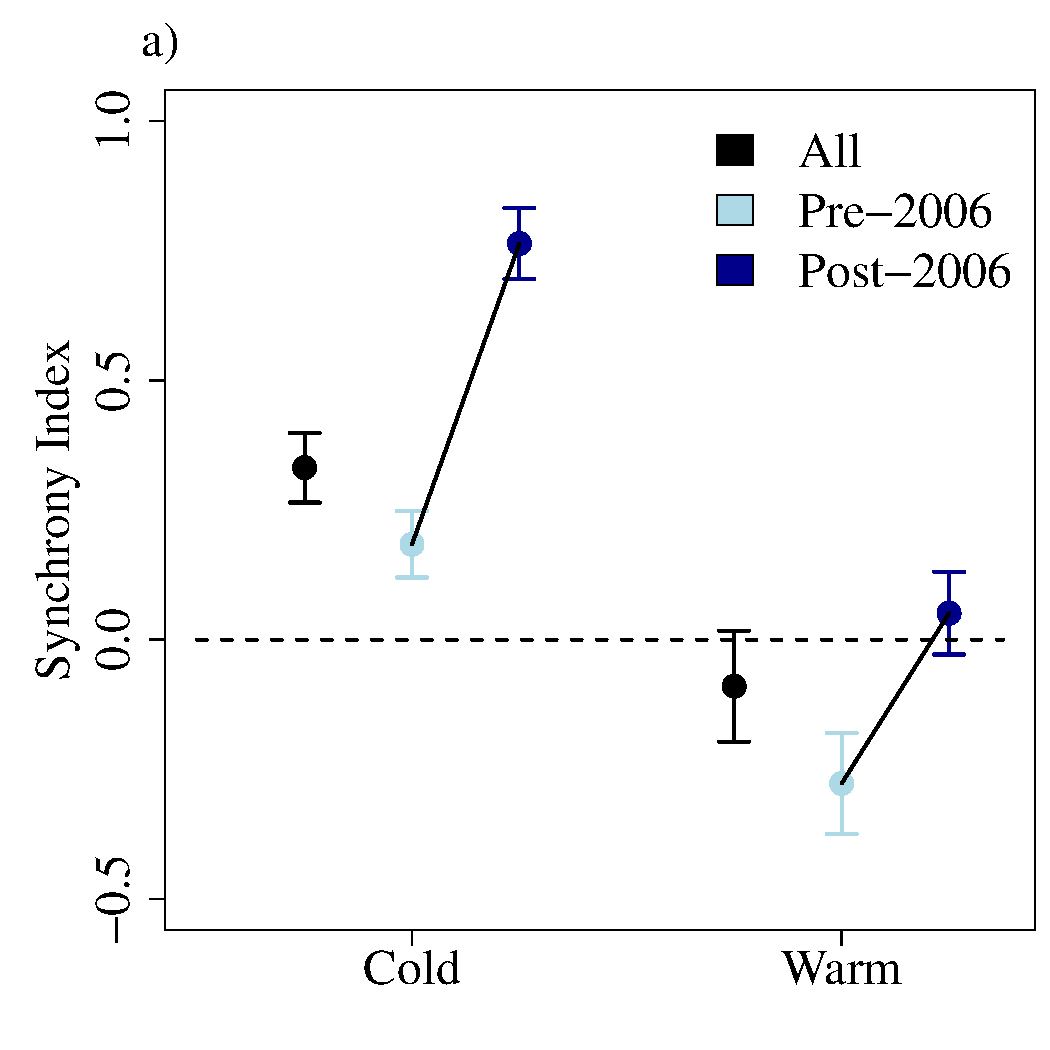
\includegraphics[width=0.55\textwidth]{gross_triad}
\par\end{centering}
\begin{centering}
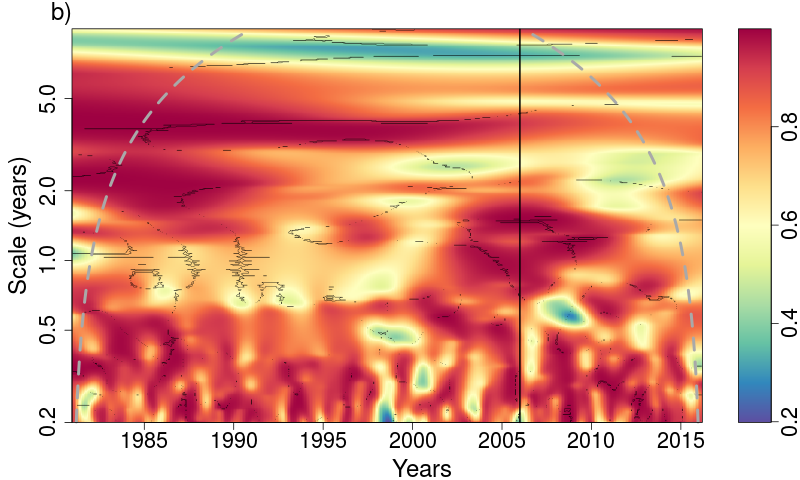
\includegraphics[width=0.7\textwidth]{wavelet_triad}
\par\end{centering}
\caption{Time-domain (a) and frequency-domain (b) synchrony analyses of the
group formed by cormorant, egret and heron\label{fig:Time-domain-(top)-and}}
\end{figure}

While compensation could be expected upon visual inspection of the
time series of the two groups formed by cormorant on the one hand,
and egret plus heron (summed as a small functional group) on the other
hand (Fig. \ref{fig:Time-series-of}), we see on Fig. \ref{fig:Time-domain-(top)-and}
that synchrony is in fact the rule around the annual scale and below,
when considering the wavelet index. We wondered if the patterns in
Fig. \ref{fig:Time-series-of} were caused by the use of a log scale,
but we found that in fact the correlation was higher rather than lower
on the log scale (Appendix 2). However, over long temporal scales ($\sim$
6 years) there seems to be some compensation, traducing a progressive
change in composition within this small community module, that was
already visible on the time series plot (Fig. \ref{fig:Time-series-of}).
There might be some compensation over very short timescale as well
(within the season), but at very specific times and the biological
mechanisms for this are unclear, since these species compete for roost
sites, a process that it unlikely to manifest at such very short timescales. 

\section*{Discussion}

Compensation was overall very rare at the yearly timescale (differentiating
between the cold and warm season). At short timescales (below the
season), and among taxonomically or functionally close species, some
compensation could be found but only at certain periods. In other
words, there was no widespread ``functional compensation'' (\textit{sensu}
\citealt{gonzalez2009causes}) \emph{within} genera or guilds at the
annual scale or below. 

Yet, summing species abundances within a guild and comparing the ``biomass
sums'' of contrasted guilds, community composition did change in
frequency in the long run; in other words, there was some compensation
\emph{between} guilds. 

Given that we compare the level of synchrony/compensation within guilds
(with many species) and between guilds (with only a handful of groups),
we checked in Appendix 3 if changing the number of ``compartments''
($n$) in the Gross $\eta$ index could affect its value: it did not.
However, we found that if two groups respond in opposite ways to a
shared driver, the stronger the response to the driver, the lesser
the compensation indicated by $\eta$ at the whole community level.
This might explain the low levels of compensation that we found at
the overall wetland bird community level (Appendix 1), in spite of the
clear presence of two groups reacting in opposite way to shared driver
(here, water levels). Analyses at several taxonomic/functional scales
are therefore warranted to be conclusive about compensation. 

We used correlation between the summed abundances of closely related species (species within the \textit{Anas} genus
vs. species within the \textit{Calidris} genus) or the summed abundances
of functionally similar species (waders vs. ducks) to uncover compensation.
The functional group classification produced much more clearly compensation
between guilds than the taxonomic classification. We expected to see
compensation at that ``functional scale'' irrespective of the season,
because the requirements of these birds are different, but here waders
and ducks were found to correlate negatively only during the cold
(wintering) season. This may be because the summer is characterized
by a broad inflow of birds, including non-resident individuals that
somehow add random variation to the community dynamics (though other
explanations are possible). 

It may be better to say that we detected ``compensation'' rather
than ``compensatory dynamics'' between bird species \citep{gonzalez2009causes}
as the observed long-term changes in species composition (more waders,
proportionally less ducks; Appendix 4) might be due to an increased inflow
of birds preferring low water levels, and outflow of birds preferring
high water levels, under an overall space constraint. In other words,
the shift in community dynamics is likely not directly due to birth
and deaths. However, despite the importance of movements and habitat
preference to the local community dynamics, there is certainly also
an influence of the regional changes in births and deaths on these
local dynamics. 

Zooming in on the cormorant-heron-egret module, we find that compensation
mostly occurs above the annual temporal scale, and predominantly in
summer as well as before 2006. This occurs because of a slow
replacement of species due to competition for resting/roosting sites in the summer
season (C. Feign�, pers. obs.), which mostly occurred before 2006. 

Overall, our results suggest to search for compensation more often\emph{
between} rather than \emph{within} functional groups, and over relatively
long timescales above that of the dominant driver (e.g., above 5 years
if the main driver is a seasonal climate). This goes against calls
to search for compensation at very short timescales \citep{vasseur2007spectral,gonzalez2009causes}
in order to filter out the effect of the main seasonal driver. Although
searching for compensation at temporal scales below the seasonal abiotic
driver (e.g., temperature) was partly motivated by studies on plankton
whose community dynamics are much faster, we could have expected compensation
to manifest also that scale here as well (e.g., monthly). Movement
of birds reacting to food availability can certainly occur that fast,
and wetlands have a finite carrying capacity, which could promote
short-term compensation. We suspect that instead, because many species
share common abiotic drivers at short temporal scales \citep{loreau_species_2008},
compensation is bound to be quite rare below the dominant temporal
scale of the environment. 

In many ways, searching for compensation using biodiversity time series
data is searching for needles in a haystack: only some specific temporal
and functional/taxonomic scales allow to see compensation whilst numerous
confounding factors make the community co-vary positively at all other
scales \citep{vasseur_synchronous_2014}. Although the knowledge of
specific biological mechanisms increasing the densities of some species
at the expense of others can help, synchrony will likely dominate
community-level time series data for closely related species, even
in species that compete strongly \citep{ranta_detecting_2008}. This
is true even in cases of known mechanisms of competition or shifts
in community composition due to abiotic changes as in this study.
We suggest that ``zooming out'' taxonomically or functionally (considering
summed abondances of dissimilar functional groups) and temporally
(considering temporal scales well above the dominant driver) may often
be the best strategy to see the compensation that will inevitably
manifest if the community-level abundance is maintained within bounds. 

\subsection*{Acknowledgements}

We thank the birdwatchers and staff of the Teich Reserve/Landes Gascogne
regional park who contributed to data collection over the years, as
well as LPO Aquitaine for helping us retrieve the raw data. The data
collection was supported by the Landes Gascogne regional park as well
as the Teich municipality, while data analysis was funded by LabEx COTE
(ANR-10-LABX-45). \\

\bibliographystyle{ecology}
\bibliography{BiblioTeich}

\end{document}
